\documentclass[10pt]{article}
\usepackage[letterpaper]{geometry}
\geometry{verbose,tmargin=1in,bmargin=1in,lmargin=1in,rmargin=1in}
\usepackage{setspace}
\usepackage{ragged2e}
\usepackage{color}
\usepackage{titlesec}
\usepackage{graphicx}
\usepackage{float}
\usepackage{mathtools}
\usepackage{amsmath}
\usepackage[font=small,labelfont=bf,labelsep=period]{caption}
\usepackage[english]{babel}
\usepackage{indentfirst}
\usepackage{array}
\usepackage{makecell}
\usepackage[usenames,dvipsnames]{xcolor}
\usepackage{multirow}
\usepackage{tabularx}
\usepackage{arydshln}
\usepackage{caption}
\usepackage{subcaption}
\usepackage{xfrac}
\usepackage{etoolbox}
\usepackage{cite}
\usepackage{url}
\usepackage{dcolumn}
\usepackage{hyperref}
\usepackage{courier}
\usepackage{url}
\usepackage{esvect}
\usepackage{commath}
\usepackage{verbatim} % for block comments
\usepackage{enumitem}
\usepackage{hyperref} % for clickable table of contents
\usepackage{braket}
\usepackage{titlesec}
\usepackage{booktabs}
\usepackage{gensymb}
\usepackage{longtable}
\usepackage{listings}
\usepackage{cancel}
\usepackage{tcolorbox}
\usepackage[mathscr]{euscript}
\lstset{
    frame=single,
    breaklines=true,
    postbreak=\raisebox{0ex}[0ex][0ex]{\ensuremath{\color{red}\hookrightarrow\space}}
}

% for circled numbers
\usepackage{tikz}
\newcommand*\circled[1]{\tikz[baseline=(char.base)]{
            \node[shape=circle,draw,inner sep=2pt] (char) {#1};}}


\titleclass{\subsubsubsection}{straight}[\subsection]

% define new command for triple sub sections
\newcounter{subsubsubsection}[subsubsection]
\renewcommand\thesubsubsubsection{\thesubsubsection.\arabic{subsubsubsection}}
\renewcommand\theparagraph{\thesubsubsubsection.\arabic{paragraph}} % optional; useful if paragraphs are to be numbered

\titleformat{\subsubsubsection}
  {\normalfont\normalsize\bfseries}{\thesubsubsubsection}{1em}{}
\titlespacing*{\subsubsubsection}
{0pt}{3.25ex plus 1ex minus .2ex}{1.5ex plus .2ex}

\makeatletter
\renewcommand\paragraph{\@startsection{paragraph}{5}{\z@}%
  {3.25ex \@plus1ex \@minus.2ex}%
  {-1em}%
  {\normalfont\normalsize\bfseries}}
\renewcommand\subparagraph{\@startsection{subparagraph}{6}{\parindent}%
  {3.25ex \@plus1ex \@minus .2ex}%
  {-1em}%
  {\normalfont\normalsize\bfseries}}
\def\toclevel@subsubsubsection{4}
\def\toclevel@paragraph{5}
\def\toclevel@paragraph{6}
\def\l@subsubsubsection{\@dottedtocline{4}{7em}{4em}}
\def\l@paragraph{\@dottedtocline{5}{10em}{5em}}
\def\l@subparagraph{\@dottedtocline{6}{14em}{6em}}
\makeatother

\newcommand{\volume}{\mathop{\ooalign{\hfil$V$\hfil\cr\kern0.08em--\hfil\cr}}\nolimits}

\setcounter{secnumdepth}{4}
\setcounter{tocdepth}{4}
\begin{document}

\title{ME 280a: HW 7}
\author{April Novak}

\maketitle

\section{Introduction and Objectives}

The purpose of this study is to describe the process for solving a 3-D diffusion-reaction equation with no time dependence, and then to describe the differences in the solution method once the problem is allowed to have time dependence. Then, a simple 1-D diffusion-reaction equation is solved as a transient case with Backward Euler (BE) time stepping.

\section{Procedure}
\label{sec:Procedure}

This section details the problem statement and mathematical method used for solving the problem.

\subsection{Theoretical Problem Statement}

Before deriving the governing equation, some preliminaries are necessary. The deformation gradient tensor \(\textbf{F}\) is used to map between two different coordinate systems. One of these coordinates frames is defined by the coordinates \(x_i\) (the present coordinates), and the other by \(X_i\) (the reference coordinates):

\begin{equation}
\label{eq:DeformationGradient}
\bar{dx}=\textbf{F}\bar{d\xi}
\end{equation}

The Jacobian \(\mathscr{J}\) is defined as the determinant of the deformation gradient tensor, and is required to transform integrals over the physical domain to the master element for application of quadrature rules:

\begin{equation}
\label{eq:Jacobian}
\mathscr{J}\equiv \det{\textbf{F}}
\end{equation}

Finally, to have a physically meaningful transformation between two coordinate frames, the Jacobian must be positive. The diffusion-reaction equation to be solved in this assignment represents a balance between the time rate of change of the concentration in a control volume with the diffusion of mass into the control volume, a reaction that either produces or removes mass from the volume, and any sources of mass:

\begin{equation}
\label{eq:DiffusionReaction}
\dot{c}=\nabla\cdot(D\nabla c)-\tau c+f
\end{equation}

where \(c\) is the concentration, an overhead dot represents differentiation in time, \(D\) the diffusion coefficient, \(\tau\) the reaction rate frequency, and \(f\) the concentration source per unit time. This problem is to be solved to determine the concentration. In general, the diffusion coefficient can be an \(n\)-th order tensor, where \(n\) is the number of spatial dimensions, but for this assignment, is assumed to be a scalar, such that the medium is isotropic.

\subsection{The Weak Form}

The weak form of Eq. \eqref{eq:DiffusionReaction} is obtained by multiplying through by a test function \(v\). Then, integrating over the body:

\begin{equation}
\label{eq:StrongForm2}
\int_{\Omega}\dot{c}vd\Omega=\int_{\Omega}\nabla\cdot(D\nabla c)vd\Omega-\int_{\Omega}\tau cvd\Omega+\int_{\Omega}fvd\Omega
\end{equation}

where \(\Omega\) is the entire domain. Applying the product rule to the diffusion term:

\begin{equation}
\int_{\Omega}\dot{c}vd\Omega=-\int_{\Omega}(\nabla v)D(\nabla c)d\Omega+\int_{\Gamma}D\nabla c\cdot\hat{n}vd\Gamma-\int_{\Omega}\tau cvd\Omega+\int_{\Omega}fvd\Omega
\end{equation}

where \(\Gamma\) is the boundary area of the domain \(\Omega\) with unit normal vector \(\hat{n}\). The boundary integral applies over the entire domain \(\Gamma=\Gamma_q\cup\Gamma_d\), where \(\Gamma_q\) is the boundary on which the mass flux is specified (Neumann boundary condition) and \(\Gamma_d\) is the boundary on which the concentration is specified (Dirichlet boundary condition). Because the value of the mass flux is unknown on the Dirichlet boundaries, specifying the third term above on the boundaries would be difficult, and hence for simplicity, the shape functions are assumed to equal zero on the Dirichlet boundaries. With this simplification:

\begin{equation}
\begin{aligned}
\int_{\Omega}\dot{c}vd\Omega=-\int_{\Omega}(\nabla v)D(\nabla c)d\Omega-\int_{\Gamma_q}qvd\Gamma-\int_{\Omega}\tau cvd\Omega+\int_{\Omega}fvd\Omega
\end{aligned}
\end{equation}

where \(q\equiv -D(\nabla c)\cdot\hat{n}\). Hence, the weak form can be stated as:

\begin{tcolorbox}
\begin{equation}
\label{eq:WeakFormQ1}
\begin{aligned}
\text{Find }c\in H^c(\Omega)\subset H^1(\Omega) \text{ so that } c|_{\Gamma_d}=\bar{c} \text{ and so that }\forall\ v \in H^v(\Omega)\subset H^1(\Omega), v|_{\Gamma_d}=0,\\
\text{and for }q\in L^2(\Gamma_q)\text{ and }f\in L^2(\Omega)\\
\int_{\Omega}\dot{c}vd\Omega=-\int_{\Omega}(\nabla v)D(\nabla c)d\Omega-\int_{\Gamma_q}qvd\Gamma-\int_{\Omega}\tau cvd\Omega+\int_{\Omega}fvd\Omega
\end{aligned}
\end{equation}
\end{tcolorbox}

where \(\bar{c}\) is the vector of known concentrations on the displacement boundary. This weak form is more general than the strong form because it does not assume twice-differentiability of the concentration. The particular weighted residual method to be applied is the Bubnov-Galerkin method, where both the solution and the weight function are expanded in the same basis functions. Hence, both the displacement and the weight function are in \(H^1(\Omega)\), the space necessary to ensure finite integrals in the weak form above. 

The space \(H^1(\Omega)\) is a Hilbert-space norm, where the 1 superscript indicates that it contains all functions whose highest finite derivative is the first derivative. This is the space from which the shape and weight functions must come because at most a first derivative is required in the weak form. For other applications, where for example, the highest derivative present in the weak form is a second derivative, then the weight and shape functions would need to be in \(H^2(\Omega)\) in order for all integrals to remain finite. In other words, \(c\) is in \(H^1(\Omega)\) if the following statement is true:

\begin{equation}
\|c\|^2_{{H}^1(\Omega)}=\int_{\Omega}\left(\frac{\partial c}{\partial x}\right)^2d\Omega+\int_{\Omega}u^2d\Omega<\infty
\end{equation}

Because the flux and source also appear in the integrals in Eq. \eqref{eq:WeakFormQ1}, there is a requirement on the space of functions from which they can inhabit. From the weak form, no differentiation of these functions is required, so they must be within \(H^0(\Omega)\), sometimes referred to as \(L^2(\Omega)\). The weak form in Eq. \eqref{eq:WeakFormQ1} is equivalent to the strong form provided that the solution is sufficiently differentiable that the higher derivatives required in the strong form are defined. Next, the specifics of the finite element implementation are given in order to specify the above to the finite element method.

\subsubsection{The Finite Element Weak Form}

This section covers the details regarding finite element implementation of Eq. \eqref{eq:WeakFormQ1}. To implement this weak form, first the solution for the concentration \(c\) and the weight function \(v\) are expanded in a series of shape functions:

\begin{equation}
\begin{aligned}
c^h=&\ \sum_{j=1}^{n_{en}}a_j\phi_j=&\textbf{N}\Phi\\
v^h=&\ \sum_{i=1}^{n_{en}}b_i\phi_i=&\textbf{N}\Psi\\
\end{aligned}
\end{equation}

where \(a\) are the expansion coefficients to be solved for, \(\phi\) are the expansion functions defined in the physical domain, and the \(h\) superscript indicates that this approximation occurs over each element, with \(n_{en}\) nodes per element. Because \(c\) is a scalar, there are \(n_{en}\) unknowns per element. The number and order of these shape functions determines the order of the finite element approximation. For convenience, the shape functions and unknowns are grouped into vectors:

\begin{equation}
\textbf{N}\equiv\begin{bmatrix}\phi_1 & \phi_2 & \phi_3 & \phi_4 & \phi_5 & \phi_6 & \phi_7 & \phi_8\end{bmatrix}
\end{equation}

\begin{equation}
\begin{aligned}
\Phi\equiv&\ \begin{bmatrix}a_1 & a_2 & a_3 & a_4 & a_5 & a_6 & a_7 & a_8\end{bmatrix}^T\\
\Psi\equiv&\ \begin{bmatrix}b_1 & b_2 & b_3 & b_4 & b_5 & b_6 & b_7 & b_8\end{bmatrix}^T\
\end{aligned}
\end{equation}

where a trilinear approximation has been assumed, such that in 3-D there are 8 nodes per element, with each node having one associated unknown. The gradient of the solution and the weight function are required in the weak form. This can be expressed conveniently as:

\begin{equation}
\begin{aligned}
\nabla c=&\ \frac{\partial c}{\partial x_1}\hat{x_1}+\frac{\partial c}{\partial x_2}\hat{x_2}+\frac{\partial c}{\partial x_3}\hat{x_3}\\
=&\ \begin{bmatrix}\frac{\partial \phi_1}{\partial x_1} & \frac{\partial \phi_2}{\partial x_1} & \frac{\partial \phi_3}{\partial x_1} & \frac{\partial \phi_4}{\partial x_1} & \frac{\partial \phi_5}{\partial x_1} & \frac{\partial \phi_6}{\partial x_1} & \frac{\partial \phi_7}{\partial x_1} & \frac{\partial \phi_8}{\partial x_1}\\
\frac{\partial \phi_1}{\partial x_2} & \frac{\partial \phi_2}{\partial x_2} & \frac{\partial \phi_3}{\partial x_2} & \frac{\partial \phi_4}{\partial x_2} & \frac{\partial \phi_5}{\partial x_2} & \frac{\partial \phi_6}{\partial x_2} & \frac{\partial \phi_7}{\partial x_2} & \frac{\partial \phi_8}{\partial x_2}\\
\frac{\partial \phi_1}{\partial x_3} & \frac{\partial \phi_2}{\partial x_3} & \frac{\partial \phi_3}{\partial x_3} & \frac{\partial \phi_4}{\partial x_3} & \frac{\partial \phi_5}{\partial x_3} & \frac{\partial \phi_6}{\partial x_3} & \frac{\partial \phi_7}{\partial x_3} & \frac{\partial \phi_8}{\partial x_3}\\ \end{bmatrix}
\Phi\\
=&\ \textbf{B}\Phi\\
\end{aligned}
\end{equation}

The gradient of the shape function is defined similarly. Inserting these approximations into the weak form:

\begin{equation}
\label{eq:FEStep1}
\int_{\Omega}\textbf{N}\dot{\Phi}\cdot(\textbf{N}\Psi)d\Omega=-\int_{\Omega}D(\textbf{B}\Psi)\cdot(\textbf{B}\Phi)d\Omega-\int_{\Gamma_q}q(\textbf{N}\Psi)d\Gamma-\int_{\Omega}\tau (\textbf{N}\Phi)\cdot(\textbf{N}\Psi)d\Omega+\int_{\Omega}f(\textbf{N}\Psi)d\Omega
\end{equation}

where it has been assumed that the shape functions are not functions of time, such that the time derivative acts only on the vector of unknowns \(\Phi\). The dot product is defined such that \(\textbf{a}\cdot\textbf{b}=\textbf{a}^T\textbf{b}\), and noting the equivalency between \(\textbf{N}\Psi\) and \((\textbf{N}\Psi)^T\)

\begin{equation}
\int_{\Omega}(\textbf{N}\Psi)^T\textbf{N}\dot{\Phi}d\Omega=-\int_{\Omega}(\textbf{B}\Psi)^TD(\textbf{B}\Phi)d\Omega-\int_{\Gamma_q}q(\textbf{N}\Psi)^Td\Gamma-\int_{\Omega}\tau (\textbf{N}\Psi)^T(\textbf{N}\Phi)d\Omega+\int_{\Omega}f(\textbf{N}\Psi)^Td\Omega
\end{equation}

Then, because \((\textbf{a}\textbf{b})^T=\textbf{b}^T\textbf{a}^T\):

\begin{equation}
\int_{\Omega}\Psi^T\textbf{N}^T\textbf{N}\dot{\Phi}d\Omega=-\int_{\Omega}\Psi^T\textbf{B}^TD(\textbf{B}\Phi)d\Omega-\int_{\Gamma_q}q\Psi^T\textbf{N}^Td\Gamma-\int_{\Omega}\tau \Psi^T\textbf{N}^T(\textbf{N}\Phi)d\Omega+\int_{\Omega}f\Psi^T\textbf{N}^Td\Omega
\end{equation}

Then, because \(\Psi^T\) appears in every term, it can effectively be cancelled (the above could be rearranged so that \(\Psi^T\) multiplies a large term, and then if that entire integral must be zero, then the integrand must also be zero). 

\begin{equation}
\int_{\Omega}\textbf{N}^T\textbf{N}\dot{\Phi}d\Omega+\int_{\Omega}\textbf{B}^TD\textbf{B}\Phi d\Omega+\int_{\Omega}\tau \textbf{N}^T\textbf{N}\Phi d\Omega=-\int_{\Gamma_q}q\textbf{N}^Td\Gamma+\int_{\Omega}f\textbf{N}^Td\Omega
\end{equation}

At this point, it is assumed that the system is in steady state. Then, the above reduces to the following:

\begin{equation}
\int_{\Omega}\textbf{B}^TD\textbf{B}\Phi d\Omega+\int_{\Omega}\tau \textbf{N}^T\textbf{N}\Phi d\Omega=-\int_{\Gamma_q}q\textbf{N}^Td\Gamma+\int_{\Omega}f\textbf{N}^Td\Omega
\end{equation}

For simplicity, the above terms can be defined as matrices:

\begin{equation}
\label{eq:FEWeakForm}
\begin{aligned}
\textbf{K}\equiv&\ \int_{\Omega}\textbf{B}^TD\textbf{B}\Phi d\Omega+\int_{\Omega}\tau \textbf{N}^T\textbf{N}\Phi d\Omega\\
\textbf{R}\equiv&\ -\int_{\Gamma_q}q\textbf{N}^Td\Gamma+\int_{\Omega}f\textbf{N}^Td\Omega\\
\end{aligned}
\end{equation}

to give the matrix system:

\begin{equation}
\textbf{K}\Phi=\textbf{R}
\end{equation}

where \(\Phi\) represents what is to be solved for over the domain. So, the weak form for the time-independent FE method (with Dirichlet boundary conditions applied using static condensation by removing them from the matrix system) is:

\begin{tcolorbox}
\begin{equation}
\label{eq:FEWeakFormFinal}
\begin{aligned}
\text{Find }\Phi\in \textbf{H}^\phi(\Omega)\subset \textbf{H}^1(\Omega) \text{ so that } \Phi|_{\Gamma_d}=\bar{\Phi} \text{ and so that }\forall\ \Psi \in \textbf{H}^\psi(\Omega)\subset \textbf{H}^1(\Omega), \Psi|_{\Gamma_d}=\textbf{0},\\
\text{and for }q\in L^2(\Gamma_q)\text{ and }f\in L^2(\Omega)\\
\int_{\Omega}\textbf{B}^TD\textbf{B}\Phi d\Omega+\int_{\Omega}\tau \textbf{N}^T\textbf{N}\Phi d\Omega=-\int_{\Gamma_q}q\textbf{N}^Td\Gamma+\int_{\Omega}f\textbf{N}^Td\Omega
\end{aligned}
\end{equation}
\end{tcolorbox}

The definitions for all the terms that appear above have been given previously. Section \ref{sec:Penalty} will show the weak form with the penalty method, while Section \ref{sec:FEElement} will show how the above is applied element-by-element.

\subsubsection{The Finite Element Weak Form - Penalty Method}
\label{sec:Penalty}

The penalty method is a means by which to apply Dirichlet boundary conditions without the tedious need to separate rows and columns from the stiffness and loading vectors. From Eq. \eqref{eq:FEWeakFormFinal}, the weak form for a finite element implementation requires that the weight functions are zero on essential boundaries. The penalty method relaxes this requirement, and adds a term to the weak form to account for violation of a Dirichlet boundary condition on a Dirichlet boundary. This method is widely-used, but is not strictly required to apply Dirichlet boundary conditions - the alternative of separating rows and columns containing known quantities, and subtracting from the load vector, can always be performed. The penalty method adds a term to the weak form of the form \(P^{*}\int_{\Gamma_d}(\textbf{N}\Psi)\cdot(\bar{c}-\textbf{N}\Phi)d\Gamma\) into Eq. \eqref{eq:FEWeakFormFinal}:

\begin{tcolorbox}
\begin{equation}
\label{eq:WeakFormPenalty}
\begin{aligned}
\text{Find }\Phi\in \textbf{H}^\phi(\Omega)\subset \textbf{H}^1(\Omega) \text{ so that } \Phi|_{\Gamma_d}=\bar{\Phi} \text{ and so that }\forall\ \Psi \in \textbf{H}^\psi(\Omega)\subset \textbf{H}^1(\Omega)\\
\text{and for }q\in L^2(\Gamma_q)\text{ and }f\in L^2(\Omega)\\
\int_{\Omega}\textbf{B}^TD\textbf{B}\Phi d\Omega+\int_{\Omega}\tau \textbf{N}^T\textbf{N}\Phi d\Omega+P^{*}\int_{\Gamma_d}\textbf{N}^T\textbf{N}\Phi d\Gamma=-\int_{\Gamma_q}q\textbf{N}^Td\Gamma+\int_{\Omega}f\textbf{N}^Td\Omega+P^{*}\int_{\Gamma_d}\textbf{N}^T\bar{c}d\Gamma
\end{aligned}
\end{equation}
\end{tcolorbox}

where \(\bar{c}\) is a vector of known concentrations on the Dirichlet boundary and \(P^{*}\) represents something like a spring constant, and is a large, positive number. A high value of this artificial spring constant will apply a traction to ``force'' the displacement boundary to be satisfied on \(\Gamma_d\), the displacement boundary. In other words, the penalty term represents a traction that enforces the Dirichlet boundary condition. This term, however, would never be applied if we still required \(\Psi|_{\Gamma_d}=\textbf{0}\), and so the kinematic restrictions on the weight functions are dropped, and they do not need to be zero on the Dirichlet boundaries. With this weak form, the matrix equation \(\textbf{K}\Phi=\textbf{R}\) remains the same, but the contents of \(\textbf{K}\) and \(\textbf{R}\) change to:

\begin{equation}
\begin{aligned}
\textbf{K}\equiv&\ \int_{\Omega}\textbf{B}^TD\textbf{B} d\Omega+\int_{\Omega}\tau \textbf{N}^T\textbf{N} d\Omega+P^{*}\int_{\Gamma_d}\textbf{N}^T\textbf{N} d\Gamma\\
\textbf{R}\equiv&\ -\int_{\Gamma_q}q\textbf{N}^Td\Gamma+\int_{\Omega}f\textbf{N}^Td\Omega+P^{*}\int_{\Gamma_d}\textbf{N}^T\bar{c}d\Gamma\\
\end{aligned}
\end{equation}

These additional penalty terms are only added for elements that are on Dirichlet boundaries, which is evident from the \(\Gamma_d\) appearing in the integral bounds.


\subsection{Finite Element Implementation}
\label{sec:FEElement}

\subsubsection{Element-by-Element Matrices and Vectors}

This section provides in explicit detail the forms of the element stiffness matrices and load vectors using the penalty method (the penalty terms could simply be dropped if needed, and hence the penalty method is discussed here to be as complete as possible). While Eq. \eqref{eq:WeakFormPenalty} holds over the entire domain, the strength of the finite element method is that the integrals in Eq. \eqref{eq:WeakFormPenalty} can be performed over each element, since the shape functions are a nodal basis such that they are only nonzero at a single node. Once assembling into the global stiffness matrix, this gives a sparse system. So, for an element \(e\), the element stiffness matrix and load vector are:

\begin{tcolorbox}
\begin{equation}
\label{eq:FEWeakForm_element}
\begin{aligned}
\textbf{K}^e\equiv&\ \int_{\Omega_e}\textbf{B}^TD\textbf{B} d\Omega+\int_{\Omega_e}\tau \textbf{N}^T\textbf{N} d\Omega+P^{*}\int_{\Gamma_{d,e}}\textbf{N}^T\textbf{N} d\Gamma\\
\textbf{R}^e\equiv&\ -\int_{\Gamma_{q,e}}q\textbf{N}^Td\Gamma+\int_{\Omega_e}f\textbf{N}^Td\Omega+P^{*}\int_{\Gamma_{d,e}}\textbf{N}^T\bar{c}d\Gamma\\
\end{aligned}
\end{equation}
\end{tcolorbox}

where \(\Gamma_{d,e}\) is the intersection of the boundary of element \(e\) with the Dirichlet boundary and \(\Gamma_{q,e}\) is the intersection of the boundary of element \(e\) with the Neumann boundary. All of these integrals are performed in the master domain using quadrature rules. This master domain is a cube defined over \(-1\leq\xi_1\leq1, -1\leq\xi_2\leq1, -1\leq\xi_3\leq1\). In order to transform between the physical and master domain, a transformation rule is needed to map between \(x,y,z\) and \(\xi_1,\xi_2,\xi_3\). This transformation rule can take many forms, but a convenient one is to simply use the shape function expansion:

\begin{equation}
x_i=\sum_{j=1}^{n_{en}}X_{i,j}\phi_j(\xi_1,\xi_2,\xi_3)
\end{equation}

where the shape functions from here forward are implied to be defined over the master element, \(X_{i,j}\) are the physical (real) coordinates, and \(i\) refers to the fact that the above expansion is assumed to apply equally for \(x_1\), \(x_2\) and \(x_3\). This mapping, which uses the shape functions as the basis for the mapping, is called a parametric map. So, all the integrals in \(\textbf{K}^e\) and \(\textbf{R}^e\) are performed over a single element by transforming the integrals to the master domain. The integrals in the physical domain are with respect to \(\bar{dx}\), and to transform them to the master domain, the deformation gradient tensor \(\textbf{F}\) defined by Eq. \eqref{eq:DeformationGradient} is used. Using the chain rule reveals the form of \(\textbf{F}\):

\begin{equation}
\label{eq:FForm}
\begin{bmatrix}x_1\\x_2\\x_3\end{bmatrix}=
\begin{bmatrix}\frac{\partial x_1}{\partial \xi_1}&\frac{\partial x_1}{\partial \xi_2}&\frac{\partial x_1}{\partial \xi_3}\\
\frac{\partial x_2}{\partial \xi_1}&\frac{\partial x_2}{\partial \xi_2}&\frac{\partial x_2}{\partial \xi_3}\\
\frac{\partial x_3}{\partial \xi_1}&\frac{\partial x_3}{\partial \xi_2}&\frac{\partial x_3}{\partial \xi_3}\end{bmatrix}
\begin{bmatrix}\xi_1\\\xi_2\\\xi_3\end{bmatrix}
\end{equation}

Or, in shorthand notation:

\begin{equation}
dx_i=F_{ij}\xi_j
\end{equation}

where suffix notation is implied. The inverse relationship is:

\begin{equation}
d\xi_j=F_{ji}dx_i=F_{ij}^{-1}dx_i
\end{equation}

The above transformation rule holds for the volume integral Jacobian - Nanson's formula must be used to transform the area integrals appearing in the element stiffness matrix and load vector to area integrals in the master domain. There is no reason that the Jacobian for the volume transformation be the same as that for the surface transformation, which is why more care must be taken here to use the correct transformation. In this case, area integrals are transformed by Nanson's rule:

\begin{equation}
\label{eq:Nanson}
dA_e=(\mathscr{J}\ \textbf{F}^{-T}\cdot\hat{N})\cdot\hat{n}d\hat{A}_e
\end{equation}

where \(\hat{n}\) is a unit normal to the master element surface (must be determined for each element on the surface), \(\hat{N}\) the normal to the physical element surface (must be determined), \(\mathscr{J}\) is the Jacobian defined in Eq. \eqref{eq:Jacobian}, and \(\textbf{F}\) is the deformation gradient tensor defined in Eq. \eqref{eq:FForm}. Then, all the integrals over areas must set one of \(\xi_i\) to \(\pm1\) to be consistent with the fact that on a surface, one of the master coordinates is held constant. So, in order to perform computations over each element, Eq. \eqref{eq:FEWeakForm_element} becomes:

\begin{equation}
\label{eq:FEWeakForm_element}
\begin{aligned}
\textbf{K}^e\equiv&\ \int_{-1}^{1}\int_{-1}^{1}\int_{-1}^{1}\textbf{B}^TD\textbf{B} |\textbf{F}|d\xi_1d\xi_2d\xi_3+\int_{-1}^{1}\int_{-1}^{1}\int_{-1}^{1}\tau \textbf{N}^T\textbf{N} |\textbf{F}|d\xi_1d\xi_2d\xi_3+P^{*}\int_{\Gamma_{d,e}}\textbf{N}^T\textbf{N} (\mathscr{J}\ \textbf{F}^{-T}\cdot\hat{N})\cdot\hat{n}d\hat{A}_e\\
\textbf{R}^e\equiv&\ -\int_{\Gamma_{q,e}}q\textbf{N}^T(\mathscr{J}\ \textbf{F}^{-T}\cdot\hat{N})\cdot\hat{n}d\hat{A}_e+\int_{-1}^{1}\int_{-1}^{1}\int_{-1}^{1}f\textbf{N}^T|\textbf{F}|d\xi_1d\xi_2d\xi_3+P^{*}\int_{\Gamma_{d,e}}\textbf{N}^T\bar{c}(\mathscr{J}\ \textbf{F}^{-T}\cdot\hat{N})\cdot\hat{n}d\hat{A}_e\\
\end{aligned}
\end{equation}

where it is implied in the area integrals that one of the spatial coordinates is set to \(\pm 1\) according to the orientation of the surface. To accurately perform the integration in the master element, everything within the integrand must also be converted to the master coordinate frame. Hence, \(\textbf{B}\) becomes:

\begin{equation}
\begin{bmatrix}\frac{\partial\xi_1}{\partial x} & \frac{\partial\xi_2}{\partial x} & \frac{\partial \xi_3}{\partial x}\\
\frac{\partial\xi_1}{\partial y} & \frac{\partial\xi_2}{\partial y} & \frac{\partial\xi_3}{\partial y}\\
\frac{\partial\xi_1}{\partial z} & \frac{\partial\xi_2}{\partial z} & \frac{\partial\xi_3}{\partial z}\\
\end{bmatrix}
\begin{bmatrix}
\frac{\partial \phi_1}{\partial \xi_1} & \frac{\partial \phi_2}{\partial \xi_1} & \frac{\partial \phi_3}{\partial \xi_1} & \frac{\partial \phi_4}{\partial \xi_1} & \frac{\partial \phi_5}{\partial \xi_1} & \frac{\partial \phi_6}{\partial \xi_1} & \frac{\partial \phi_7}{\partial \xi_1} & \frac{\partial \phi_8}{\partial \xi_1}\\
\frac{\partial \phi_1}{\partial \xi_2} & \frac{\partial \phi_2}{\partial \xi_2} & \frac{\partial \phi_3}{\partial \xi_2} & \frac{\partial \phi_4}{\partial \xi_2} & \frac{\partial \phi_5}{\partial \xi_2} & \frac{\partial \phi_6}{\partial \xi_2} & \frac{\partial \phi_7}{\partial \xi_2} & \frac{\partial \phi_8}{\partial \xi_2}\\
\frac{\partial \phi_1}{\partial \xi_3} & \frac{\partial \phi_2}{\partial \xi_3} & \frac{\partial \phi_3}{\partial \xi_3} & \frac{\partial \phi_4}{\partial \xi_3} & \frac{\partial \phi_5}{\partial \xi_3} & \frac{\partial \phi_6}{\partial \xi_3} & \frac{\partial \phi_7}{\partial \xi_3} & \frac{\partial \phi_8}{\partial \xi_3}\\ 
\end{bmatrix}
=
\textbf{B}
\end{equation}

As mentioned previously, it is implied that all shape functions appearing in this section are defined over the master domain. So, \(\textbf{B}\) is replaced by \(\textbf{F}^{-1}\mathscr{B}\), where \(\mathscr{B}\) is the second matrix on the LHS above. This leads to the following element-wise stiffness matrix and load vector:

\begin{equation}
\label{eq:FEWeakForm_element2}
\begin{aligned}
\textbf{K}^e\equiv&\ \int_{-1}^{1}\int_{-1}^{1}\int_{-1}^{1}(\textbf{F}^{-1}\mathscr{B})^TD(\textbf{F}^{-1}\mathscr{B}) |\textbf{F}|d\xi_1d\xi_2d\xi_3+\int_{-1}^{1}\int_{-1}^{1}\int_{-1}^{1}\tau \textbf{N}^T\textbf{N} |\textbf{F}|d\xi_1d\xi_2d\xi_3+\quad\\
&\ P^{*}\int_{\Gamma_{d,e}}\textbf{N}^T\textbf{N} (\mathscr{J}\ \textbf{F}^{-T}\cdot\hat{N})\cdot\hat{n}d\hat{A}_e\\
\textbf{R}^e\equiv&\ -\int_{\Gamma_{q,e}}q\textbf{N}^T(\mathscr{J}\ \textbf{F}^{-T}\cdot\hat{N})\cdot\hat{n}d\hat{A}_e+\int_{-1}^{1}\int_{-1}^{1}\int_{-1}^{1}f\textbf{N}^T|\textbf{F}|d\xi_1d\xi_2d\xi_3+\quad\\
&\ P^{*}\int_{\Gamma_{d,e}}\textbf{N}^T\bar{c}(\mathscr{J}\ \textbf{F}^{-T}\cdot\hat{N})\cdot\hat{n}d\hat{A}_e\\
\end{aligned}
\end{equation}

The trilinear brick shape functions (in the master domain) are defined in Eq. \eqref{eq:Bricks}. The unit normals are of length 3, and are oriented such that the correct dimensions are obtained in the matrix and load integrals above. All the integrals above are performed using quadrature. To integrate in higher than a single dimension using a Gaussian quadrature rule, simply apply the rule in each direction. So, in 1-D, where a single loop sums over all the quadrature points, three loops are needed to sum over the \(\xi_1,\xi_2,\xi_3\) directions. For instance, the integrals above, in quadrature form, are:

\begin{equation}
\label{eq:FEWeakForm_element3}
\begin{aligned}
\textbf{K}^e=\sum_{q=1}^g\sum_{r=1}^g\sum_{s=1}^gw_qw_gw_s\left\{(\textbf{F}^{-1}\mathscr{B})^TD(\textbf{F}^{-1}\mathscr{B}) |\textbf{F}|+\tau \textbf{N}^T\textbf{N} |\textbf{F}|\right\} +\quad\\
\sum_{r=1}^g\sum_{s=1}^gw_gw_s\left\{P^{*}\textbf{N}^T\textbf{N} (\mathscr{J}\ \textbf{F}^{-T}\cdot\hat{N})\cdot\hat{n}\right\}\\
\ \\
\textbf{R}^e\equiv\sum_{q=1}^g\sum_{r=1}^g\sum_{s=1}^gw_qw_gw_sf\textbf{N}^T|\textbf{F}|+\quad\\
\sum_{r=1}^g\sum_{s=1}^gw_gw_s\left\{-q\textbf{N}^T(\mathscr{J}\ \textbf{F}^{-T}\cdot\hat{N})\cdot\hat{n}+P^{*}\textbf{N}^T\bar{c}(\mathscr{J}\ \textbf{F}^{-T}\cdot\hat{N})\cdot\hat{n}\right\}\\
\end{aligned}
\end{equation}

where \(g\) is the number of quadrature points, where the same quadrature rule has been assumed to be applied in each spatial dimension. It is implied that in the area integrals, \(d\hat{A}_e\) refers to one of \(d\xi_1d\xi_2\), \(d\xi_2d\xi_3, d\xi_3d\xi_1\), depending on the particular surface. To be as explicit as possible, there are essentially four types of elements. The element stiffness matrix and load vector for each of these possible combinations is shown below for completeness.

\begin{enumerate}
\item an element on the interior (no displacement or traction boundaries)

\begin{equation}
\begin{aligned}
\textbf{K}^e\equiv&\ \int_{-1}^{1}\int_{-1}^{1}\int_{-1}^{1}(\textbf{F}^{-1}\mathscr{B})^TD(\textbf{F}^{-1}\mathscr{B}) |\textbf{F}|d\xi_1d\xi_2d\xi_3+\int_{-1}^{1}\int_{-1}^{1}\int_{-1}^{1}\tau \textbf{N}^T\textbf{N} |\textbf{F}|d\xi_1d\xi_2d\xi_3\\
\textbf{R}^e\equiv&\ \int_{-1}^{1}\int_{-1}^{1}\int_{-1}^{1}f\textbf{N}^T|\textbf{F}|d\xi_1d\xi_2d\xi_3\\
\end{aligned}
\end{equation}

\item an element on the boundary with only displacement boundaries

\begin{equation}
\begin{aligned}
\textbf{K}^e\equiv&\ \int_{-1}^{1}\int_{-1}^{1}\int_{-1}^{1}(\textbf{F}^{-1}\mathscr{B})^TD(\textbf{F}^{-1}\mathscr{B}) |\textbf{F}|d\xi_1d\xi_2d\xi_3+\int_{-1}^{1}\int_{-1}^{1}\int_{-1}^{1}\tau \textbf{N}^T\textbf{N} |\textbf{F}|d\xi_1d\xi_2d\xi_3+\quad\\
&\ P^{*}\int_{\Gamma_{d,e}}\textbf{N}^T\textbf{N} (\mathscr{J}\ \textbf{F}^{-T}\cdot\hat{N})\cdot\hat{n}d\hat{A}_e\\
\textbf{R}^e\equiv&\ \int_{-1}^{1}\int_{-1}^{1}\int_{-1}^{1}f\textbf{N}^T|\textbf{F}|d\xi_1d\xi_2d\xi_3+P^{*}\int_{\Gamma_{d,e}}\textbf{N}^T\bar{c}(\mathscr{J}\ \textbf{F}^{-T}\cdot\hat{N})\cdot\hat{n}d\hat{A}_e\\
\end{aligned}
\end{equation}

\item an element on the boundary with only traction boundaries

\begin{equation}
\begin{aligned}
\textbf{K}^e\equiv&\ \int_{-1}^{1}\int_{-1}^{1}\int_{-1}^{1}(\textbf{F}^{-1}\mathscr{B})^TD(\textbf{F}^{-1}\mathscr{B}) |\textbf{F}|d\xi_1d\xi_2d\xi_3+\int_{-1}^{1}\int_{-1}^{1}\int_{-1}^{1}\tau \textbf{N}^T\textbf{N} |\textbf{F}|d\xi_1d\xi_2d\xi_3\\
\textbf{R}^e\equiv&\ -\int_{\Gamma_{q,e}}q\textbf{N}^T(\mathscr{J}\ \textbf{F}^{-T}\cdot\hat{N})\cdot\hat{n}d\hat{A}_e+\int_{-1}^{1}\int_{-1}^{1}\int_{-1}^{1}f\textbf{N}^T|\textbf{F}|d\xi_1d\xi_2d\xi_3\\
\end{aligned}
\end{equation}

\item an element on the boundary with both displacement and traction boundaries

\begin{equation}
\begin{aligned}
\textbf{K}^e\equiv&\ \int_{-1}^{1}\int_{-1}^{1}\int_{-1}^{1}(\textbf{F}^{-1}\mathscr{B})^TD(\textbf{F}^{-1}\mathscr{B}) |\textbf{F}|d\xi_1d\xi_2d\xi_3+\int_{-1}^{1}\int_{-1}^{1}\int_{-1}^{1}\tau \textbf{N}^T\textbf{N} |\textbf{F}|d\xi_1d\xi_2d\xi_3+\quad\\
&\ P^{*}\int_{\Gamma_{d,e}}\textbf{N}^T\textbf{N} (\mathscr{J}\ \textbf{F}^{-T}\cdot\hat{N})\cdot\hat{n}d\hat{A}_e\\
\textbf{R}^e\equiv&\ -\int_{\Gamma_{q,e}}q\textbf{N}^T(\mathscr{J}\ \textbf{F}^{-T}\cdot\hat{N})\cdot\hat{n}d\hat{A}_e+\int_{-1}^{1}\int_{-1}^{1}\int_{-1}^{1}f\textbf{N}^T|\textbf{F}|d\xi_1d\xi_2d\xi_3+\quad\\
&\ P^{*}\int_{\Gamma_{d,e}}\textbf{N}^T\bar{c}(\mathscr{J}\ \textbf{F}^{-T}\cdot\hat{N})\cdot\hat{n}d\hat{A}_e\\
\end{aligned}
\end{equation}
\end{enumerate}

Care must be taken for determining if an element is on a Dirichlet boundary. If it is, then penalty terms must be added, and if not, the penalty terms are absent. So, whether or not the penalty method is used, there is some amount of bookkeeping required to record which nodes correspond to Dirichlet boundaries.

\subsubsection{Global-Local Transformation}

After all computations over the elements are complete, all the local stiffness matrices and load vectors must be organized into the global stiffness matrix and load vector. The placement of local matrices into the global matrix is performed using a connectivity matrix that relates the local node numbers to the global node numbers. A connectivity matrix is usually organized so that each row corresponds to a single element. Then, each column in that row refers to each local node in that element, and the information held in the connectivity matrix are the global node numbers relating to the local node numbers. For example, for a 2-D domain with four elements, and global node numbering beginning in the bottom left corner and moving up to the top right corner, the connectivity matrix (also called the location matrix \textbf{LM} in this document) has the following form:

\begin{equation}
\textbf{LM}=\begin{bmatrix}
1 & 2 & 5 & 4\\
2 & 3 & 6 & 5\\
4 & 5 & 8 & 7\\
5 & 6 & 9 & 8\\
\end{bmatrix}
\end{equation}

where the local nodes are numbered in a counterclockwise manner beginning from the bottom left node. Then, for example, the second row in the global stiffness matrix would be assembled as:

\begin{equation}
\textbf{K}(2,:)=\begin{bmatrix}
k_{2,1}^{e=1}, & k_{2,2}^{e=1}+k_{1,1}^{e=2}, & k_{1,2}^{e=2}, & k_{2,4}^{e=1}, & k_{1,4}^{e=2}+k_{2,3}^{e=1}, & k_{1,3}^{e=2}, & 0, & 0, & 0\\
\end{bmatrix}
\end{equation}

\subsection{Shape Functions}

The shape functions for 3-D finite elements are a natural extension of the shape functions used in lower dimensions. Trilinear elements, or 3-D linear elements, are used for the remainder of this assignment. This choice of shape functions represents a nodal basis, since the shape functions go to zero at all nodes except for the node for which they are defined. The trilinear shape functions are:

\begin{equation}
\label{eq:Bricks}
\begin{aligned}
\phi_1(\xi_1,\xi_2,\xi_3)=\frac{1}{8}(1-\xi_1)(1-\xi_2)(1-\xi_3)\\
\phi_2(\xi_1,\xi_2,\xi_3)=\frac{1}{8}(1+\xi_1)(1-\xi_2)(1-\xi_3)\\
\phi_3(\xi_1,\xi_2,\xi_3)=\frac{1}{8}(1+\xi_1)(1+\xi_2)(1-\xi_3)\\
\phi_4(\xi_1,\xi_2,\xi_3)=\frac{1}{8}(1-\xi_1)(1+\xi_2)(1-\xi_3)\\
\phi_5(\xi_1,\xi_2,\xi_3)=\frac{1}{8}(1-\xi_1)(1-\xi_2)(1+\xi_3)\\
\phi_6(\xi_1,\xi_2,\xi_3)=\frac{1}{8}(1+\xi_1)(1-\xi_2)(1+\xi_3)\\
\phi_7(\xi_1,\xi_2,\xi_3)=\frac{1}{8}(1+\xi_1)(1+\xi_2)(1+\xi_3)\\
\phi_8(\xi_1,\xi_2,\xi_3)=\frac{1}{8}(1-\xi_1)(1+\xi_2)(1+\xi_3)\\
\end{aligned}
\end{equation}

\section{Mesh Generator}

This section discusses the mesh generator used to mesh the tubular ``S'' structure given in the assignment, and is largely a repeat of the mesh used for assignment 5, except that it has been modified to work for an unknown that is a scalar quantity, rather than a vector quantity. While the mesh is the same as that for assignment 5, the location matrix now does not need to have an associated matrix that relates the three unknowns for each node to their position in the global matrix (here, there is only one unknown per node). The meshing begins in each \(\theta\)-chunk. For the circular cross-section structure, the \(x\) and \(y\) coordinates are related to each other by:

\begin{equation}
\label{eq:xy}
x^2+y^2=r
\end{equation}

where \(r\) is the inner radius of the tubular structure. Each piece in the circumferential direction is defined according to \(\theta\), where \(0\leq\theta\leq2\pi\) defines the ``slice'' parallel to \(\vv{e}_r\). The generation of the mesh is based on determining the coordinates of each node. The first node is assigned to the first ``slice'' for \(\theta=0\). In the discussion of the mesh generator, ``slice'' refers to each plane for which there exists a hollowed annulus (that is meshed according to the number of layers and circumferential points). \(\Theta\) is the angle referring to the circumferential angle, while \(\theta\) refers to the angle in each slice. The overall algorithm for generating the coordinates for the mesh is as follows:

\begin{enumerate}
\item Begin with slice for \(\Theta=0\). Beginning then for \(\theta=0\), move counterclockwise around the first layer (inner surface of the tube). Increment \(\theta\) in units of \(2\pi/N_c\), and for each \(\theta\), assign the \(x\) and \(y\) coordinates according to Eq. \eqref{eq:xy}. 
\item After finishing the inner layer, increase \(r\) by \(dt\), where \(dt\) is the thickness of each layer, to move to the next layer, then repeat step 1. 
\item Repeat steps 1 and 2 until all layers in each slice have been meshed, where for each layer, \(dt\) is added. 
\item Now that a slice has been meshed, repeat for all slices. This requires determining the \(x,y,z\) centers for each new slice. This is performed by sweeping through \(\Theta\). The \(y\) coordinate is \(y=0\) for all points, while the \(x\) coordinate continually increases moving from slice to slice, and the \(z\) coordinate is positive for the left half of the tube, and negative for the right half of the tube. 
\item Now that all slices have been meshed, the mesh looks like as follows for \(N_c=8, N_\theta=8, N_t=3\). 

\begin{figure}[H]
  \centering
  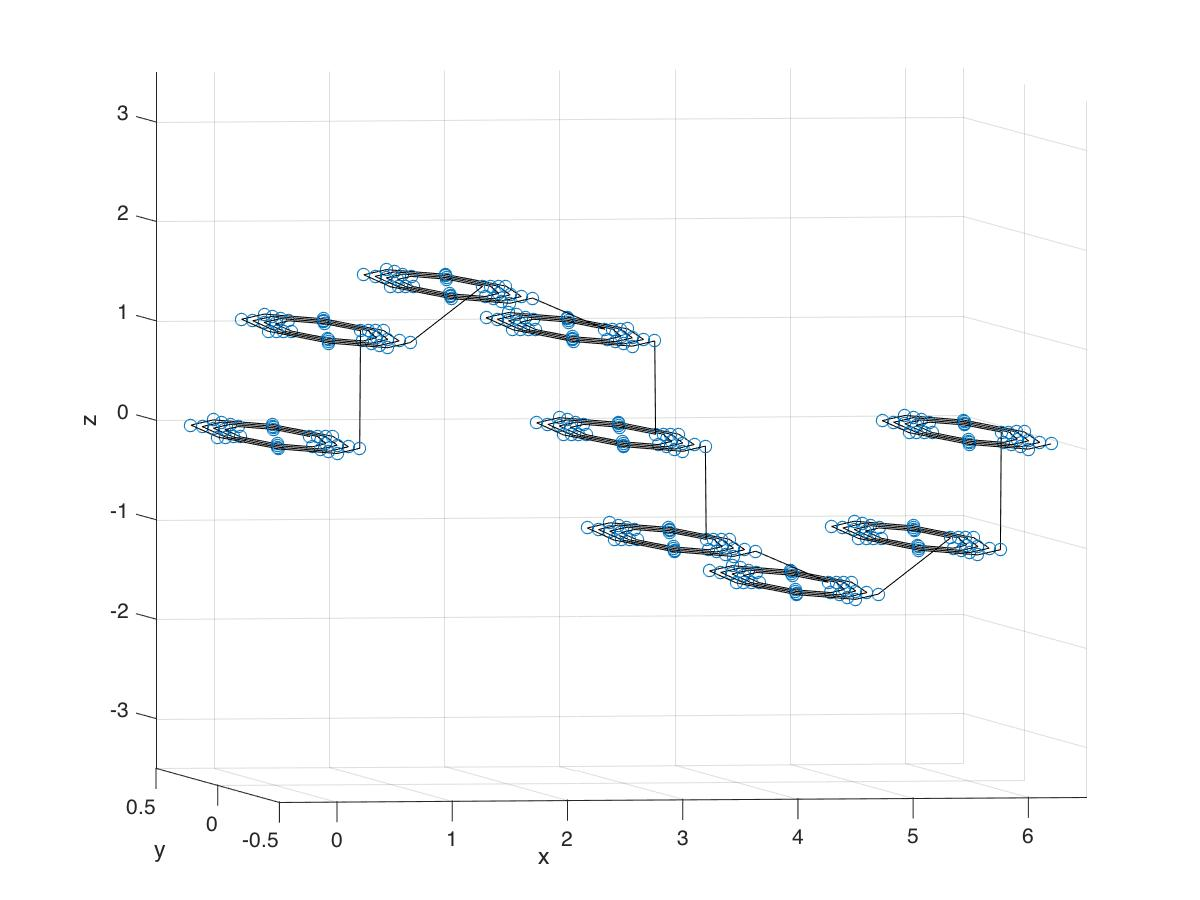
\includegraphics[width=10cm]{NoTilt.jpg}
  \caption{Mesh for \(N_c=8, N_\theta=8, N_t=3\) with no tilt to the slices. Lines connect each coordinate for better visuality.}
\end{figure}

The next step is to rotate the slices appropriately through the angle \(\Theta\) for each slice so that a tubular structure is formed. Only the \(x\) and \(z\) coordinates must be modified. To perform the tilt, the following quantities are computed using trigonometry:

\begin{equation}
\begin{aligned}
w=\sin{(\pi/2-\Theta)}(r+dt)\cos{(\theta)}/\sin{(pi/2)}\\
h = w\sin{(\Theta)}\\
p = w\cos{(\Theta)}\\
\end{aligned}
\end{equation}

To tilt the z-coordinate, for points in the first and fourth quadrant of each slice:

\begin{equation}
z_{new} = z - (-1)^{tube}h
\end{equation}

And for points in the second and third quadrant of each slice:

\begin{equation}
z_{new} = z + (-1)^{tube}h
\end{equation}

where \(tube\) is a variable indicating whether or not the slice is in the left or right half of the tube. For the left half of the tube, \(tube=1\), and in the right half, \(tube=2\).

\item Then, tilt the x-coordinates. For points in the first and fourth quadrants of each slice:

\begin{equation}
x_{new} = x + p
\end{equation}

And for points in the second and third quadrants of each slice:

\begin{equation}
x_{new} = x - p
\end{equation}

\item Finally, tilt the slices that exactly align with the peak and valley of the tube (for odd numbers of \(N_\theta\), this would not be performed). For the slices that align with the peaks and for nodes in the first and fourth quadrants, adjust the \(z\) coordinates according to:

\begin{equation}
z_{new} = z - (r+dt)\cos{(\theta)}
\end{equation}

And for points in the second and third quadrants:

\begin{equation}
z_{new} = z + (r+dt)\cos{(\theta)}
\end{equation}

The \(x\)-coordinates are adjusted by simply setting all of them to the centroid coordinate for that slice. 
\end{enumerate}

This process is fairly complicated, and reveals why meshing software is so valuable. The process here is left fairly general that it can apply for any values of \(N_\theta, N_c, N_t\), but any slight change in the geometry completely invalidates the program. The final mesh for \(N_c=8, N_\theta=8, N_t=3\) is shown below. This mesh is shown because the requested mesh with only \(N_c=4\) is relatively difficult to perceive in a 3-D plot in Matlab, so the following plot better reveals the mesh. Lines are drawn between each coordinate.

\begin{figure}[H]
  \centering
  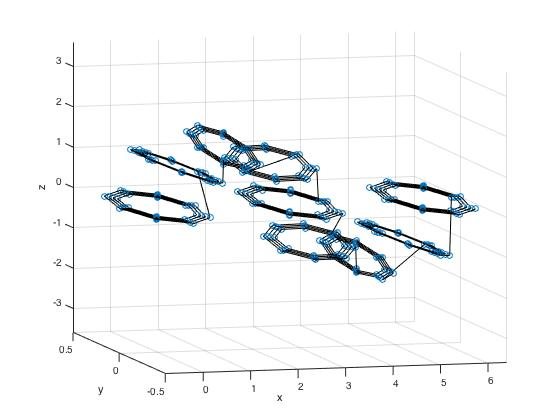
\includegraphics[width=10cm]{RefinedMesh.jpg}
  \caption{Mesh for \(N_c=8, N_\theta=8, N_t=3\). Lines connect each coordinate for better visuality.}
\end{figure}

The coarser mesh, for \(N_c=4, N_\theta=8, N_t=3\) is shown below, again with lines connecting each coordinate for better visibility.

\begin{figure}[H]
  \centering
  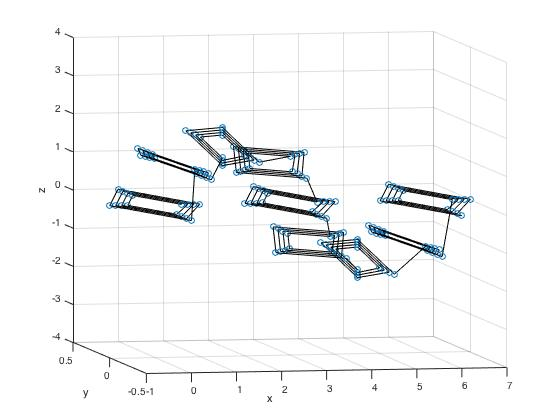
\includegraphics[width=10cm]{CoarseMesh.jpg}
  \caption{Mesh for \(N_c=4, N_\theta=8, N_t=3\). Lines connect each coordinate for better visuality.}
\label{fig:CoarseMesh}
\end{figure}

The mesh in Fig. \ref{fig:CoarseMesh} is shown below without the lines connecting each coordinate.

\begin{figure}[H]
  \centering
  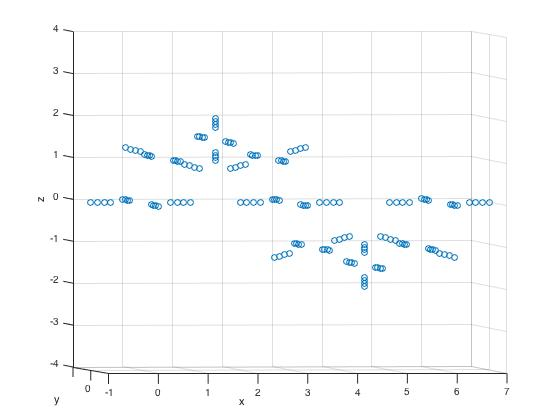
\includegraphics[width=10cm]{CoarseMeshNoLines.jpg}
  \caption{Mesh for \(N_c=4, N_\theta=8, N_t=3\).}
\end{figure}

Note that this assignment did not provide the dimensions of the tube, so I assumed that the inner radius of each arch was 1, the radius of the inner hole of the tube 0.3, and the thickness of the tube 0.2.

\subsection{The Connectivity Matrix}

In order for this mesh to be useful for finite element implementation, a connectivity function must be defined to relate the local node numbering to the global node numbering. The mesh generated numbers the global nodes according to the order in which they were generated. For instance, the first 8 nodes are in the inner layer of the first slice, the next 8 are in the second layer of the first slice, and so on for the first slice. Then, moving to the next \(\Theta\) slice, the node numbering again begins on the inside of the tube and moves counterclockwise in layers until reaching the outside of the tube. This is shown schematically in the figures above by the black lines connecting the coordinates \textit{in the order in which the coordinates are generated}.

The connectivity matrix is an \(N\times8\) matrix, where \(N\) is the total number of elements and 8 is the number of local nodes per element (linear elements are assumed). The local node numbering is performed according to a clockwise fashion. The following schematic shows the node numbering, where the left portion shows the front face, and the right portion shows the back face, all while looking at the front face (i.e. the back face is not written with the perspective of looking at the outward-facing portion of the back face).

\begin{equation}
\begin{aligned}
4 -- 3 & \quad\quad & 8 -- 7\\
2 -- 1 & \quad\quad & 6 -- 5\\
\end{aligned}
\end{equation}

So, for each slice, the nodes on the face of each element can be determined using a numbering scheme that follows the order in which the nodes were defined. Beginning with \(\theta=0\), and moving counterclockwise, the local nodes are numbered, moving progressively outwards in the layers until reaching the last node for a particular slice. 

There are \(N_t\cdot N_c\cdot N_\theta\) total elements. For each slice, the nodes are numbered moving counterclockwise, beginning at the same node that is meshed first. After each layer is complete, the numbering moves to the next layer in the same fashion. Once an entire slice is complete, the next slice is also meshed. This defines only the \textit{frontal} node numberings shown in the above equation. For example, for \(N_\theta=2, N_t=3, N_c=4\), the connectivity matrix \(\textbf{LM}\) looks like the following \textit{before} the nodes on the backs of the first 12 elements are related to the nodes on the fronts of the next 12 elements.

\begin{equation}
\textbf{LM}=
\begin{bmatrix}
1 & 2 & 5 & 6 & 0 & 0 & 0 & 0\\
2 & 3 & 6 & 7 & 0 & 0 & 0 & 0\\
3 & 4 & 7 & 8 & 0 & 0 & 0 & 0\\
4 & 1 & 8 & 5 & 0 & 0 & 0 & 0\\
5 & 6 & 9 & 10 & 0 & 0 & 0 & 0\\
6 & 7 & 10 & 11 & 0 & 0 & 0 & 0\\
7 & 8 & 11 & 12 & 0 & 0 & 0 & 0\\
8 & 5 & 12 & 9 & 0 & 0 & 0 & 0\\
9 & 10 & 13 & 14 & 0 & 0 & 0 & 0\\
10 & 11 & 14 & 15 & 0 & 0 & 0 & 0\\
11 & 12 & 15 & 16 & 0 & 0 & 0 & 0\\
12 & 9 & 16 & 13 & 0 & 0 & 0 & 0\\
17 & 18 & 21 & 22 & 0 & 0 & 0 & 0\\
18 & 19 & 22 & 23 & 0 & 0 & 0 & 0\\
19 & 20 & 23 & 24 & 0 & 0 & 0 & 0\\
20 & 17 & 24 & 21 & 0 & 0 & 0 & 0\\
21 & 22 & 25 & 26 & 0 & 0 & 0 & 0\\
22 & 23 & 26 & 27 & 0 & 0 & 0 & 0\\
23 & 24 & 27 & 28 & 0 & 0 & 0 & 0\\
24 & 21 & 28 & 25 & 0 & 0 & 0 & 0\\
25 & 26 & 29 & 30 & 0 & 0 & 0 & 0\\
26 & 27 & 30 & 31 & 0 & 0 & 0 & 0\\
27 & 28 & 31 & 32 & 0 & 0 & 0 & 0\\
28 & 25 & 32 & 29 & 0 & 0 & 0 & 0\\
33 & 34 & 37 & 38 & 0 & 0 & 0 & 0\\
34 & 35 & 38 & 39 & 0 & 0 & 0 & 0\\
35 & 36 & 39 & 40 & 0 & 0 & 0 & 0\\
36 & 33 & 40 & 37 & 0 & 0 & 0 & 0\\
37 & 38 & 41 & 42 & 0 & 0 & 0 & 0\\
38 & 39 & 42 & 43 & 0 & 0 & 0 & 0\\
39 & 40 & 43 & 44 & 0 & 0 & 0 & 0\\
40 & 37 & 44 & 41 & 0 & 0 & 0 & 0\\
41 & 42 & 45 & 46 & 0 & 0 & 0 & 0\\
42 & 43 & 46 & 47 & 0 & 0 & 0 & 0\\
43 & 44 & 47 & 48 & 0 & 0 & 0 & 0\\
44 & 41 & 48 & 45 & 0 & 0 & 0 & 0\\
\end{bmatrix}
\end{equation}

This is not the final form for the connectivity matrix (a.k.a. location matrix). Because the slices lay exactly on top of one another, the front nodes of the second slice are exactly the back nodes on the previous slice. With this knowledge, the back nodes for each element can be assigned based on the frontal nodes of the following slice. Then, the last \(N_cN_t\) rows in the location matrix above can be deleted, since they refer to the frontal nodes of a slice that does not technically exist (there are only 2 slices, but 3 planes defining those slices). With this information, the final form of the location matrix becomes, for \(N_\theta=2, N_t=3, N_c=4\) for example:

\begin{equation}
\textbf{LM}=
\begin{bmatrix}
1 & 2 & 5 & 6 & 17 & 18 & 21 & 22\\
2 & 3 & 6 & 7 & 18 & 19 & 22 & 23\\
3 & 4 & 7 & 8 & 19 & 20 & 23 & 24\\
4 & 1 & 8 & 5 & 20 & 17 & 24 & 21\\
5 & 6 & 9 & 10 & 21 & 22 & 25 & 26\\
6 & 7 & 10 & 11 & 22 & 23 & 26 & 27\\
7 & 8 & 11 & 12 & 23 & 24 & 27 & 28\\
8 & 5 & 12 & 9 & 24 & 21 & 28 & 25\\
9 & 10 & 13 & 14 & 25 & 26 & 29 & 30\\
10 & 11 & 14 & 15 & 26 & 27 & 30 & 31\\
11 & 12 & 15 & 16 & 27 & 28 & 31 & 32\\
12 & 9 & 16 & 13 & 28 & 25 & 32 & 29\\
17 & 18 & 21 & 22 & 33 & 34 & 37 & 38\\
18 & 19 & 22 & 23 & 34 & 35 & 38 & 39\\
19 & 20 & 23 & 24 & 35 & 36 & 39 & 40\\
20 & 17 & 24 & 21 & 36 & 33 & 40 & 37\\
21 & 22 & 25 & 26 & 37 & 38 & 41 & 42\\
22 & 23 & 26 & 27 & 38 & 39 & 42 & 43\\
23 & 24 & 27 & 28 & 39 & 40 & 43 & 44\\
24 & 21 & 28 & 25 & 40 & 37 & 44 & 41\\
25 & 26 & 29 & 30 & 41 & 42 & 45 & 46\\
26 & 27 & 30 & 31 & 42 & 43 & 46 & 47\\
27 & 28 & 31 & 32 & 43 & 44 & 47 & 48\\
28 & 25 & 32 & 29 & 44 & 41 & 48 & 45\\
\end{bmatrix}
\end{equation}

Each row in the location matrix corresponds to an elements, and each column to a local node number, so that \(LM(1,4)\) indicates the global node number of local node number 4 in element 1. This method is extended to the case for \(N_\theta=8, N_c=4, N_t=3\), where the purpose of the previous discussion for a fewer number of circumferential elements was simply to illustrate the process by which the location matrix is generated. So, for the problem statement in this homework assignment (\(N_\theta=8, N_c=4, N_t=3\)):

\begin{equation}
\label{eq:LMFinalForm}
\textbf{LM}=
\begin{bmatrix}LM_1 \\ LM_2\end{bmatrix}
\end{equation}

where, in order to be able to print the matrix, the following components are defined to simply be stacked on top of each other as in Eq. \eqref{eq:LMFinalForm}.

\begin{equation}
LM_1=
\begin{bmatrix}
1 & 2 & 5 & 6 & 17 & 18 & 21 & 22\\
2 & 3 & 6 & 7 & 18 & 19 & 22 & 23\\
3 & 4 & 7 & 8 & 19 & 20 & 23 & 24\\
4 & 1 & 8 & 5 & 20 & 17 & 24 & 21\\
5 & 6 & 9 & 10 & 21 & 22 & 25 & 26\\
6 & 7 & 10 & 11 & 22 & 23 & 26 & 27\\
7 & 8 & 11 & 12 & 23 & 24 & 27 & 28\\
8 & 5 & 12 & 9 & 24 & 21 & 28 & 25\\
9 & 10 & 13 & 14 & 25 & 26 & 29 & 30\\
10 & 11 & 14 & 15 & 26 & 27 & 30 & 31\\
11 & 12 & 15 & 16 & 27 & 28 & 31 & 32\\
12 & 9 & 16 & 13 & 28 & 25 & 32 & 29\\
17 & 18 & 21 & 22 & 33 & 34 & 37 & 38\\
18 & 19 & 22 & 23 & 34 & 35 & 38 & 39\\
19 & 20 & 23 & 24 & 35 & 36 & 39 & 40\\
20 & 17 & 24 & 21 & 36 & 33 & 40 & 37\\
21 & 22 & 25 & 26 & 37 & 38 & 41 & 42\\
22 & 23 & 26 & 27 & 38 & 39 & 42 & 43\\
23 & 24 & 27 & 28 & 39 & 40 & 43 & 44\\
24 & 21 & 28 & 25 & 40 & 37 & 44 & 41\\
25 & 26 & 29 & 30 & 41 & 42 & 45 & 46\\
26 & 27 & 30 & 31 & 42 & 43 & 46 & 47\\
27 & 28 & 31 & 32 & 43 & 44 & 47 & 48\\
28 & 25 & 32 & 29 & 44 & 41 & 48 & 45\\
33 & 34 & 37 & 38 & 49 & 50 & 53 & 54\\
34 & 35 & 38 & 39 & 50 & 51 & 54 & 55\\
35 & 36 & 39 & 40 & 51 & 52 & 55 & 56\\
36 & 33 & 40 & 37 & 52 & 49 & 56 & 53\\
37 & 38 & 41 & 42 & 53 & 54 & 57 & 58\\
38 & 39 & 42 & 43 & 54 & 55 & 58 & 59\\
39 & 40 & 43 & 44 & 55 & 56 & 59 & 60\\
40 & 37 & 44 & 41 & 56 & 53 & 60 & 57\\
41 & 42 & 45 & 46 & 57 & 58 & 61 & 62\\
42 & 43 & 46 & 47 & 58 & 59 & 62 & 63\\
43 & 44 & 47 & 48 & 59 & 60 & 63 & 64\\
44 & 41 & 48 & 45 & 60 & 57 & 64 & 61\\
49 & 50 & 53 & 54 & 65 & 66 & 69 & 70\\
50 & 51 & 54 & 55 & 66 & 67 & 70 & 71\\
51 & 52 & 55 & 56 & 67 & 68 & 71 & 72\\
52 & 49 & 56 & 53 & 68 & 65 & 72 & 69\\
53 & 54 & 57 & 58 & 69 & 70 & 73 & 74\\
54 & 55 & 58 & 59 & 70 & 71 & 74 & 75\\
55 & 56 & 59 & 60 & 71 & 72 & 75 & 76\\
56 & 53 & 60 & 57 & 72 & 69 & 76 & 73\\
57 & 58 & 61 & 62 & 73 & 74 & 77 & 78\\
58 & 59 & 62 & 63 & 74 & 75 & 78 & 79\\
59 & 60 & 63 & 64 & 75 & 76 & 79 & 80\\
60 & 57 & 64 & 61 & 76 & 73 & 80 & 77\\
65 & 66 & 69 & 70 & 81 & 82 & 85 & 86\\
\end{bmatrix}
\end{equation}

\begin{equation}
LM_2=
\begin{bmatrix}
66 & 67 & 70 & 71 & 82 & 83 & 86 & 87\\
67 & 68 & 71 & 72 & 83 & 84 & 87 & 88\\
68 & 65 & 72 & 69 & 84 & 81 & 88 & 85\\
69 & 70 & 73 & 74 & 85 & 86 & 89 & 90\\
70 & 71 & 74 & 75 & 86 & 87 & 90 & 91\\
71 & 72 & 75 & 76 & 87 & 88 & 91 & 92\\
72 & 69 & 76 & 73 & 88 & 85 & 92 & 89\\
73 & 74 & 77 & 78 & 89 & 90 & 93 & 94\\
74 & 75 & 78 & 79 & 90 & 91 & 94 & 95\\
75 & 76 & 79 & 80 & 91 & 92 & 95 & 96\\
76 & 73 & 80 & 77 & 92 & 89 & 96 & 93\\
81 & 82 & 85 & 86 & 97 & 98 & 101 & 102\\
82 & 83 & 86 & 87 & 98 & 99 & 102 & 103\\
83 & 84 & 87 & 88 & 99 & 100 & 103 & 104\\
84 & 81 & 88 & 85 & 100 & 97 & 104 & 101\\
85 & 86 & 89 & 90 & 101 & 102 & 105 & 106\\
86 & 87 & 90 & 91 & 102 & 103 & 106 & 107\\
87 & 88 & 91 & 92 & 103 & 104 & 107 & 108\\
88 & 85 & 92 & 89 & 104 & 101 & 108 & 105\\
89 & 90 & 93 & 94 & 105 & 106 & 109 & 110\\
90 & 91 & 94 & 95 & 106 & 107 & 110 & 111\\
91 & 92 & 95 & 96 & 107 & 108 & 111 & 112\\
92 & 89 & 96 & 93 & 108 & 105 & 112 & 109\\
97 & 98 & 101 & 102 & 113 & 114 & 117 & 118\\
98 & 99 & 102 & 103 & 114 & 115 & 118 & 119\\
99 & 100 & 103 & 104 & 115 & 116 & 119 & 120\\
100 & 97 & 104 & 101 & 116 & 113 & 120 & 117\\
101 & 102 & 105 & 106 & 117 & 118 & 121 & 122\\
102 & 103 & 106 & 107 & 118 & 119 & 122 & 123\\
103 & 104 & 107 & 108 & 119 & 120 & 123 & 124\\
104 & 101 & 108 & 105 & 120 & 117 & 124 & 121\\
105 & 106 & 109 & 110 & 121 & 122 & 125 & 126\\
106 & 107 & 110 & 111 & 122 & 123 & 126 & 127\\
107 & 108 & 111 & 112 & 123 & 124 & 127 & 128\\
108 & 105 & 112 & 109 & 124 & 121 & 128 & 125\\
113 & 114 & 117 & 118 & 129 & 130 & 133 & 134\\
114 & 115 & 118 & 119 & 130 & 131 & 134 & 135\\
115 & 116 & 119 & 120 & 131 & 132 & 135 & 136\\
116 & 113 & 120 & 117 & 132 & 129 & 136 & 133\\
117 & 118 & 121 & 122 & 133 & 134 & 137 & 138\\
118 & 119 & 122 & 123 & 134 & 135 & 138 & 139\\
119 & 120 & 123 & 124 & 135 & 136 & 139 & 140\\
120 & 117 & 124 & 121 & 136 & 133 & 140 & 137\\
121 & 122 & 125 & 126 & 137 & 138 & 141 & 142\\
122 & 123 & 126 & 127 & 138 & 139 & 142 & 143\\
123 & 124 & 127 & 128 & 139 & 140 & 143 & 144\\
124 & 121 & 128 & 125 & 140 & 137 & 144 & 141\\
\end{bmatrix}
\end{equation}

\section{Computational Cost}

The cost of a 3-D finite element simulation of a scalar-valued equation such as the diffusion-reaction equation results in element stiffness matrices of size \(8\times8\) when using trilinear shape functions. For a cubical mesh, with \(M\times M\) elements, there are \((M+1)^3\) total unknowns in the mesh, so the global stiffness matrix is of size \(((M+1)^3)\times((M+1)^3)\). If the symmetry of the local stiffness matrices is taken into account (they will always be symmetric for linear differential equations so long as the Bubnov-Galerkin approach is used), then the required storage per element drops from 64 to 28. 

If the Conjugate Gradient (CG) method is used to solve the matrix system \(\textbf{K}\textbf{a}=\textbf{R}\), then this represents repeated application of a \(8\times8\) matrix and a \(8\times1\) vector, which is an \(\mathscr{O}(N)\) operation. This is performed for each iteration, so the cost for the CG method scales as \(\mathscr{O}(IN)\), where \(I\) is the number of iterations needed to reach a particular tolerance in the solve.

The cost of a solve refers to both the storage required and the number of floating point operations required. There are three ways to perform the storage for a mesh consisting of \(M\times M\times M\) linear elements:

\begin{enumerate}
\item Direct storage - all zeros are stored, and no shortcuts are made by saving element-by-element. This requires \(((M+1)^3)\times((M+1)^3)\approx M^6\)
\item Element-by-element storage: no zeros are stored. This requires \(8\times8\times M^3=64M^3\)
\item Element-by-element storage, taking advantage of the symmetry of the element stiffness matrices. This requires \(28M^3\)
\end{enumerate} 

So, the storage scales cubically when using element-by-element storage as opposed to direct storage. The number of floating point operations is also significantly reduced when using an iterative solver. The total number of unknowns is \((M+1)^3\), so the ratio of the direct solver (Gaussian elimination) to the CG method is:

\begin{equation}
\frac{\mathscr{O}(N^3)}{I\mathscr{O}(N)}=\frac{\left((M+1)^3\right)^2}{I}=\frac{(M+1)^6}{I}
\end{equation}

where \(N=(M+1)^3\) is the total number of unknowns. For \(N_t\times N_c\times N_\theta\) elements, there are \((N_t+1)N_c(N_\theta+1)\) total nodes. So, if there are 3 unknowns per node, and if a CG solver takes \(I\mathscr{O}(N)\) operations, then the total number of operations required is:

\begin{equation}
\text{Operations with CG method}=I(N_t+1)N_c(N_\theta+1)
\end{equation}
 
 where \(I\) is the number of iterations.

\section{Appendix}

This section contains the complete code used in this assignment. 

\subsection{\texttt{MeshGenerator.m}}
This program generates the mesh and connectivity matrix.
\lstinputlisting[language=Matlab]{MeshGenerator.m}

\end{document}